% pain
% consider toggling word wrap in your editor
\documentclass[11pt, titlepage]{article}
\usepackage[utf8]{inputenc}
\usepackage[english]{babel}


% bibliography
\usepackage[
backend=biber,
style=numeric,
sorting=ynt
]{biblatex}
\addbibresource{refs.bib}

% useful packages
\usepackage{amsmath}
\usepackage{graphicx}
\usepackage[colorlinks=true, allcolors=blue]{hyperref}

\usepackage{listings}
\usepackage{xcolor}

% US paper
\usepackage[letterpaper, margin=1in]{geometry}
\usepackage{setspace}
\onehalfspacing

% move page number
\usepackage{fancyhdr}
\pagestyle{fancy}
\fancyfoot{}
\rfoot{\thepage}

\definecolor{codegreen}{rgb}{0,0.6,0}
\definecolor{codegray}{rgb}{0.5,0.5,0.5}
\definecolor{codepurple}{rgb}{0.58,0,0.82}
\definecolor{backcolour}{rgb}{0.95,0.95,0.92}

\lstdefinestyle{mystyle}{
    backgroundcolor=\color{backcolour},   
    commentstyle=\color{codegreen},
    keywordstyle=\color{magenta},
    numberstyle=\tiny\color{codegray},
    stringstyle=\color{codepurple},
    basicstyle=\ttfamily\footnotesize,
    breakatwhitespace=false,         
    breaklines=true,
    captionpos=b,
    keepspaces=true,
    numbers=left,
    numbersep=5pt,
    showspaces=false,
    showstringspaces=false,
    showtabs=false,
    tabsize=2
}

\lstset{style=mystyle}

\title{Simulating the Effectiveness of Physics-informed Machine Learning in Nonlinear Model Predictive Control for Robotic Manipulators}
\author{Asa Paparo}
\date{}

\begin{document}

\maketitle

\begin{abstract}

Existing methods of robotic motion planning rely on numerical optimization to generate control actions within constraints. One of the most successful methods of control has been Model Predictive Control (MPC), which continuously replans a trajectory by solving an online optimization problem. This means that for high dimension dynamical systems, the computational cost of MPC can rapidly become prohibitive. Physics Informed Neural Networks (PINNs) allow for the data driven creation and solving of high dimensional differential equations. Existing research has made progress in combining them, but lacks rigor and code optimization. In this paper, I develop an efficient NMPC implementation that relies on a PINN to plan movements. Then, I set up and integrate the controller with a state of the art simulation to demonstrate its effectiveness for a 7 DoF robotic arm. This development presents a significant advancement for fields that employ mobile robotics, such as manufacturing and search/rescue.
\end{abstract}

\section{Introduction}

Robotic manipulation is an area of high importance as global manufacturing increasingly relies on automation to accomplish tasks that would typically be done by humans. Advances in robotics and machine learning promise to be integral in the fourth industrial revolution, improving efficiency and worker safety \cite{industry_4.0}. Specifically, the advancement and effectiveness of industrial robotic systems is central to a developed nation's prosperity and economy. Due to high domestic costs and restrictions, offshore manufacturing is utilized by companies seeking to minimize cost of production. To improve economic conditions without worsening worker conditions, the United States must rely on robotic manufacturing \cite{manufacturing_prosperity}. Additionally, search and rescue presents a major opportunity for robotics to improve by making it safer and more efficient \cite{search_rescue}. For medicine, surgical robots can accomplish tasks with more precision and safety than their human counterparts \cite{2, 3, 4, 5}.

A primary goal of the field of control theory is the efficient and constrained control of complex dynamical systems. A highly popular approach for this is Model Predictive Control, which relies on continuously replanning a trajectory over a specific horizon \cite{mpc_industry}.

% \cite{youm2023imitating}
% shap review
%     - us government priorities:
%     - semi automated production
%     - make national production economically feasible
%     - well educated laborors, robots work with them

%     - developed a new framework that is applicable
    
%     - antibiotics production
%     - very important production
%     - microchips, taiwan, etc
%     - focus on relevant industries

%     - cutting edge of robotics surgery is nano robotic surgery
%     - nanorobots swarm etc
%     - in order to exploit specifics, it would be highly beneficial to modify architecture in X ways
%     - claim adaptive ml algorithms are needed
%     - adaptive algorithms for smart manufacturing and adaptive ml



    % Current methods of robotic manipulation rely on predefined systems and control algorithms to function effectively. \cite{underactuated} This is a effective in most scenarios. However, it requires retuning for any change to the system. In consumer or high risk situations, it may be impractical to retune systems periodically to account for changes to the physical hardware. In this paper, I propose an alternative paradigm using physics-informed machine learning to correct for changes to the system on the fly.

    % The goal of this experiment is to examine the effectiveness <develop a new generation> of PINN (Physics Informed Neural Networks) in adapting the model of a system on the fly. This would enable the dynamic updating of control algorithms, given little prior knowledge about external conditions. For example, a manipulator should be able to grasp any arbitrary load and continue to plan trajectories effectively. In order to test this, I derive the governing equations of motion for a simple 2-DOF arm system and use drake \cite{drake} to run discrete simulations of MPC and trajectory planning for this arm. To verify my hypothesis, I modify the load attatched to the manipulator midway through the simulation and record the new effectiveness of controlling it.


    % Robotic manipulation is an area of high importance as global manufacturing increasingly relies on automation to accomplish tasks that would typically be done by humans. Advances in machine learning promise to be as impactful as an industrial revolution, with potential to deliver widespread benefits to civilization.\cite{ai_on_industrial} Specifically, advances in robotic automation for manufacturing and medicine have potential to reshape their industries for the better. In the case of manufacturing, this allows for significantly greater productivity and worker safety. For medicine, surgical robots can accomplish tasks with more precision and safety than their human counterparts. \cite{2, 3, 4, 5} Automation in manufacturing is also critical for the prosperity and improvement of our modern society. For example, relevance in the global economy is viewed as core to American national security, and automation is an essential part in that \cite{6}. Such importance is further exacerbated by declining birth rates in industrialized nations, which means a smaller workforce to support a growing aging population \cite{tandf2}. Because of this, advances in robotic automation are essential in overcoming global challenges and improving the standard of living around the world.
    
    % Robotic trajectory optimization is a well known field, however, implementations often suffer from relatively long compute times for numerical optimization. Additionally, successful throwing implementations for rigid robotic arms exist. However, they all 


    % analytical dynamics


\section{Methods}

\subsection{Nonlinear Model Predictive Control (NMPC)}

Model predictive control \cite{MPC} and its nonlinear variation rely on an algorithm of several steps.
\begin{enumerate}
    \item Create an optimized trajectory from current to target states over the specified horizon
    \item Follow the first discrete state within the larger trajectory
    \item Repeat with the new state
\end{enumerate}

Derivation from \cite{Illinois_motion}

\begin{equation}
J(x,u) = \int_0^\infty L(x(t),u(t),t) dt.
\label{eq:CostFunctional}
\end{equation}

\begin{equation}
\begin{gathered}
x^\star, u^\star = \arg \min_{x,u} J(x,u) \text{ such that} \\
\dot{x}(t) = f(x(t),u(t)) \text{ for all }t  \quad \text{(Dynamics constraint)} \\
x(0) = x_0 \quad \text{(Initial state)}
\end{gathered}
\label{eq:OptimalControl}
\end{equation}

\subsection{Physics Informed Neural Networks (PINNs)}
\subsection{Simulation}

To create an effective simulation for system, I use Drake \cite{drake}, a framework for controlling and simulating robotic systems. The specific system I control is a 7 degrees of freedom KUKA iiwa arm, documented in MIT Manipulation \cite{manipulation}

\begin{figure}
\centering
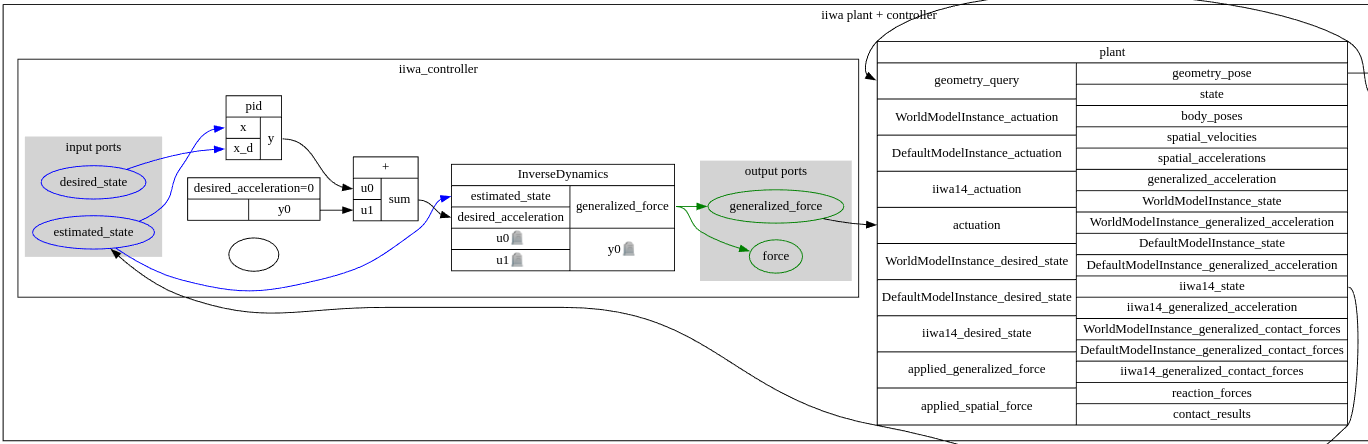
\includegraphics[width=1\linewidth]{diagram.png}
\caption{\label{fig:diagram}A flow diagram of the PID controller and system.}
\end{figure}


\begin{figure}
\centering
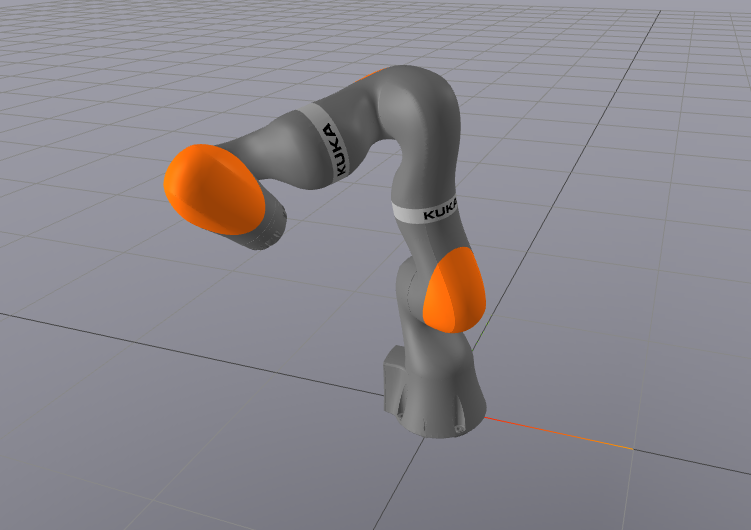
\includegraphics[width=0.25\linewidth]{iiwa.png}
\caption{\label{fig:iiwa}A visualization of the simulation, using Meshcat and the iiwa14 urdf file.}
\end{figure}

\begin{lstlisting}[language=Python]
meshcat = StartMeshcat()
def run_simulation():
    meshcat.Delete()
    meshcat.DeleteAddedControls()
    
    builder = DiagramBuilder()

    # Adds both MultibodyPlant and the SceneGraph, and wires them together.
    plant, scene_graph = AddMultibodyPlantSceneGraph(builder, time_step=1e-4)
    # Note that we parse into both the plant and the scene_graph here.
    iiwa_model = Parser(plant, scene_graph).AddModelsFromUrl(
        "package://drake/manipulation/models/iiwa_description/sdf/iiwa14_no_collision.sdf"
    )[0]
    plant.WeldFrames(plant.world_frame(), plant.GetFrameByName("iiwa_link_0"))
    plant.Finalize()

    # Adds the MeshcatVisualizer and wires it to the SceneGraph.
    visualizer = MeshcatVisualizer.AddToBuilder(builder, scene_graph, meshcat)

    # pid controller
    kp = [100] * plant.num_positions()
    ki = [1] * plant.num_positions()
    kd = [20] * plant.num_positions()
    iiwa_controller = builder.AddSystem(
        InverseDynamicsController(plant, kp, ki, kd, False)
    )
    iiwa_controller.set_name("iiwa_controller")

    # Connect ports
    builder.Connect(
        plant.get_state_output_port(iiwa_model),
        iiwa_controller.get_input_port_estimated_state()
    )
    builder.Connect(
        iiwa_controller.get_output_port_control(),
        plant.get_actuation_input_port()
    )
    diagram = builder.Build()
    diagram.set_name("with iiwa controller")

    context = diagram.CreateDefaultContext()
    plant_context = plant.GetMyMutableContextFromRoot(context)
    q0 = np.array([-1.57, 0.1, 0, -1.2, 0, 1.6, 2])
    x0 = np.hstack((q0, 2 * q0))
    plant.SetPositions(plant_context, q0)
    iiwa_controller.GetInputPort("desired_state").FixValue(
        iiwa_controller.GetMyMutableContextFromRoot(context), x0
    )
    print(context)
    # plant.SetPositions(plant_context, [-1.57, 0.1, 0, -1.2, 0, 1.6, 0])
    # plant.get_actuation_input_port().FixValue(plant_context, np.zeros(7))

    simulator = Simulator(diagram, context)
    simulator.set_target_realtime_rate(1.0)

    meshcat.StartRecording()
    simulator.AdvanceTo(10.0)
    meshcat.StopRecording()
    meshcat.PublishRecording()

    display(
    SVG(pydot.graph_from_dot_data(diagram.GetGraphvizString())[0].create_svg())
)

\end{lstlisting}
This code

\section{Discussion}

In the future, 

\section{Conclusion}

% \begin{thebibliography}{unsrt}
%     \bibitem{ai_on_industrial}
%         https://arxiv.org/pdf/2011.03044.pdf
%     \bibitem{Roach}
%         Roach, N., Venkadesan, M., Rainbow, M. et al. Elastic energy storage in the shoulder and the evolution of high-speed throwing in Homo . Nature 498, 483–486 (2013). https://doi.org/10.1038/nature12267
%     \bibitem{2}
%         https://nvlpubs.nist.gov/nistpubs/eab/nist.eab.1.pdf
%     \bibitem{3}
%         https://www.tandfonline.com/doi/abs/10.1080/10408363.2018.1561640
%     \bibitem{4}
%         https://onlinelibrary.wiley.com/doi/abs/10.1002/rcs.408
%     \bibitem{5}
%         https://www.mckinsey.de/~/media/McKinsey/Business%20Functions/Operations/Our%20Insights/Human%20plus%20machine%20A%20new%20era%20of%20automation%20in%20manufacturing/Human-plus-machine-A-new-era-of-automation-in-manufacturing.pdf
%     \bibitem{6}
%         https://escholarship.org/content/qt0tw0h6kg/qt0tw0h6kg.pdf

%     \bibitem{tandf2}
%         https://www.tandfonline.com/doi/full/10.1080/09513590701718364


%     \bibitem{pinns}
%         https://towardsdatascience.com/physics-informed-neural-networks-pinns-an-intuitive-guide-fff138069563


\printbibliography

\end{document}
